\onecolumn
\appendix
% \begin{algorithm}[tb]
%     \caption{JitRL: Test-Time Policy Optimization}
%     \label{alg:jitrl}
%  \begin{algorithmic}
%     \STATE {\bfseries Input:} State $s$, Memory $\mathcal{M}$, LLM $\pi_\theta$, hyperparameters $k, \beta, \lambda, \alpha$
%     \STATE {\bfseries Output:} Action $a$

%     \STATE \textcolor{blue}{\textit{// Step 1: Retrieve similar experiences}}
%     \STATE $\mathcal{N}(s) \leftarrow$ Top-k neighbors from $\mathcal{M}$ by Jaccard$(s, si)$

%     \STATE \textcolor{blue}{\textit{// Step 2: Estimate state value (baseline)}}
%     \STATE $V(s) \leftarrow \frac{1}{|\mathcal{N}(s)|}\sum_{(s_i, a_i, G_i) \in \mathcal{N}(s)} G_i$

%     \STATE \textcolor{blue}{\textit{// Step 3: Construct augmented candidate set}}
%     \STATE Get LLM candidates $\mathcal{C}_{\text{LLM}}$ with logits $z(a,s)$
%     \STATE $\mathcal{A}_{\text{mem}} \leftarrow \{a_i : (s_i, a_i, G_i) \in \mathcal{N}(s)\}$
%     \STATE $\mathcal{C} \leftarrow \mathcal{C}_{\text{LLM}} \cup \mathcal{A}_{\text{mem}}$
%     \FOR{$a \in \mathcal{A}_{\text{mem}} \setminus \mathcal{C}_{\text{LLM}}$}
%         \STATE $z(s,a) \leftarrow 0$ \hfill \textcolor{gray}{\textit{// Initialize logit for memory-only actions}}
%     \ENDFOR

%     \STATE \textcolor{blue}{\textit{// Step 4: Estimate Q-value for each candidate}}
%     \FOR{$a \in \mathcal{C}$}
%         \STATE $\mathcal{N}(s, a) \leftarrow \{(s_i, a_i, G_i) \in \mathcal{N}(s) : a_i = a\}$
%         \IF{$|\mathcal{N}(s, a)| > 0$}
%             \STATE $Q(s,a) \leftarrow \frac{1}{|\mathcal{N}(s,a)|}\sum_{(s_i, a_i, G_i) \in \mathcal{N}(s,a)} G_i$ \hfill \textcolor{gray}{\textit{// Known action}}
%         \ELSE
%             \IF{$\text{rand}() < \lambda$}
%                 \STATE $Q(s,a) \leftarrow V(s) + \alpha / |\mathcal{N}(s)|$ \hfill \textcolor{gray}{\textit{// Exploration bonus}}
%             \ELSE
%                 \STATE $Q(s,a) \leftarrow 0$ \hfill \textcolor{gray}{\textit{// Neutral value}}
%             \ENDIF
%         \ENDIF
%     \ENDFOR

%     \STATE \textcolor{blue}{\textit{// Step 5: Compute normalized advantage}}
%     \FOR{$a \in \mathcal{C}$}
%         \STATE $A(s,a) \leftarrow Q(s,a) - V(s)$
%     \ENDFOR
%     \STATE $A_{\max} \leftarrow \max_{a' \in \mathcal{C}}|A(s,a')| + \epsilon$
%     \FOR{$a \in \mathcal{C}$}
%         \STATE $\tilde{A}(s,a) \leftarrow A(s,a) / A_{\max}$
%     \ENDFOR

%     \STATE \textcolor{blue}{\textit{// Step 6: Closed-form policy update}}
%     \FOR{$a \in \mathcal{C}$}
%         \STATE $z'(s,a) \leftarrow z(s,a) + \beta \cdot \tilde{A}(s,a)$
%     \ENDFOR

%     \STATE \textbf{Return} Sample from $\text{Softmax}(z'(\cdot, s))$
%  \end{algorithmic}
%  \end{algorithm}


\begin{algorithm}[h]
    \caption{JitRL: Test-Time Policy Optimization}
    \label{alg:jitrl}
 \begin{algorithmic}
    \STATE {\bfseries Input:} LLM $\pi_\theta$, hyperparameters $k, \beta, \lambda, \alpha, \gamma$
    \STATE {\bfseries Initialize:} Memory $\mathcal{M} \leftarrow \emptyset$

    \FOR{each episode}
        \STATE Initialize trajectory $\tau \leftarrow []$
        \WHILE{episode not done}
            \STATE Observe state $o$; abstract to $s \leftarrow \text{AbstractState}(o)$

            \STATE \textcolor{blue}{\textit{// Step 1: Retrieve similar experiences}}
            \STATE $\mathcal{N}(s) \leftarrow$ Top-$k$ neighbors from $\mathcal{M}$ by Jaccard$(s, s_i)$

            \STATE \textcolor{blue}{\textit{// Step 2: Estimate state value (baseline)}}
            \STATE $V(s) \leftarrow \frac{1}{|\mathcal{N}(s)|}\sum_{(s_i, a_i, G_i) \in \mathcal{N}(s)} G_i$

            \STATE \textcolor{blue}{\textit{// Step 3: Construct augmented candidate set}}
            \STATE Get LLM candidates $\mathcal{C}_{\text{LLM}}$ with logits $z(s,a)$

            \STATE $\mathcal{C} \leftarrow \mathcal{C}_{LLM} \cup \{ a_i : (s_i, a_i, G_i) \in \mathcal{N}(s) \}$.
            \FOR{$a \in \mathcal{C} \setminus \mathcal{C}_{\text{LLM}}$}
                \STATE $z(s,a) \leftarrow 0$ \hfill \textcolor{gray}{\textit{// Initialize logit for memory-only actions}}
            \ENDFOR

            \STATE \textcolor{blue}{\textit{// Step 4: Estimate value for each candidate}}
            \FOR{$a \in \mathcal{C}$}
                \STATE $\mathcal{N}(s, a) \leftarrow \{(s_i, a_i, G_i) \in \mathcal{N}(s) : a_i = a\}$
                \IF{$|\mathcal{N}(s, a)| > 0$}
                    \STATE $Q(s,a) \leftarrow \frac{1}{|\mathcal{N}(s,a)|}\sum_{(s_i, a_i, G_i) \in \mathcal{N}(s,a)} G_i$ \hfill \textcolor{gray}{\textit{// Known action}}
                \ELSE
                    \IF{$\text{rand}() < \lambda$}
                        \STATE $Q(s,a) \leftarrow V(s) + \alpha / |\mathcal{N}(s)|$ \hfill \textcolor{gray}{\textit{// Exploration bonus}}
                    \ELSE
                        \STATE $Q(s,a) \leftarrow 0$ \hfill \textcolor{gray}{\textit{// Neutral value}}
                    \ENDIF
                \ENDIF
            \ENDFOR

            \STATE \textcolor{blue}{\textit{// Step 5: Compute normalized advantage}}
            \FOR{$a \in \mathcal{C}$}
                \STATE $A(s,a) \leftarrow Q(s,a) - V(s)$
            \ENDFOR
            \STATE $A_{\max} \leftarrow \max_{a' \in \mathcal{C}}|A(s,a')| + \epsilon$
            \FOR{$a \in \mathcal{C}$}
                \STATE $\tilde{A}(s,a) \leftarrow A(s,a) / (A_{\max}+\epsilon)$
            \ENDFOR

            \STATE \textcolor{blue}{\textit{// Step 6: Closed-form policy update}}
            \FOR{$a \in \mathcal{C}$}
                \STATE $z'(s,a) \leftarrow z(s,a) + \beta \cdot \tilde{A}(s,a)$
            \ENDFOR

            \STATE Sample $a \sim \text{Softmax}(z')$; append $(s, a)$ to $\tau$
        \ENDWHILE

        \STATE \textcolor{blue}{\textit{// Step 7: Memory update after episode ends}}
        \STATE $\{r_t\}_{t=0}^{T} \leftarrow \text{Evaluator}(\tau)$
        \FOR{$t = 0$ \textbf{to} $T$}
            \STATE $G_t \leftarrow \sum_{u=t}^{T} \gamma^{u-t} r_u$
            \STATE $\mathcal{M} \leftarrow \mathcal{M} \cup \{(s_t, a_t, G_t)\}$
        \ENDFOR
    \ENDFOR
 \end{algorithmic}
 \end{algorithm}

\section{Algorithm}
\label{app:alg}
Algorithm ~\ref{alg:jitrl} shows the overall algorithm of JitRL.
 
\section{Derivation of the Optimal Closed-Form Solution}
\label{app:derivation}

In this appendix, we provide the full derivation for Theorem \ref{thm:closed_form}. We show that the additive logit update rule is the exact solution to the KL-constrained advantage maximization problem.

\subsection{Problem Formulation}

Recall our optimization objective defined in Eq.~\eqref{eq:optimization_objective}. We seek a policy distribution $\pi'$ that maximizes the expected estimated advantage while maintaining a bounded KL divergence from the reference policy $\pi_{\theta}$:

\begin{equation}
    \max_{\pi'} \quad \mathbb{E}_{a \sim \pi'} [\widehat A(s,a)] - \frac{1}{\beta} D_{KL}(\pi' || \pi_{\theta}).
\end{equation}

Subject to the probability constraint that the distribution must sum to 1:
\begin{equation}
    \sum_{a } \pi'(a) = 1.
\end{equation}

Expanding the expectation and KL divergence terms, the objective function $J(\pi')$ can be written as:

\begin{equation}
    J(\pi') = \sum_{a} \pi'(a) \widehat A(s,a) - \frac{1}{\beta} \sum_{a} \pi'(a) \log \frac{\pi'(a)}{\pi_{\theta}(a)}.
\end{equation}

\subsection{Lagrangian Optimization}

To solve this constrained optimization problem, we introduce a Lagrange multiplier $\lambda$ for the summation constraint. The Lagrangian function $\mathcal{L}(\pi', \lambda)$ is:

\begin{equation}
    \mathcal{L}(\pi', \lambda) = \sum_{a} \pi'(a) \widehat A(s,a) - \frac{1}{\beta} \sum_{a} \pi'(a) (\log \pi'(a) - \log \pi_{\theta}(a)) + \lambda \left( \sum_{a} \pi'(a) - 1 \right).
\end{equation}

We take the derivative of $\mathcal{L}$ with respect to $\pi'(a)$ for a specific action $a$ and set it to zero:

\begin{equation}
    \frac{\partial \mathcal{L}}{\partial \pi'(a)} = \widehat A(s,a) - \frac{1}{\beta} (1 + \log \pi'(a) - \log \pi_{\theta}(a)) + \lambda = 0.
\end{equation}

Rearranging the terms to solve for $\log \pi'(a)$:

\begin{equation}
    \frac{1}{\beta} \log \pi'(a) = \widehat A(s,a) + \frac{1}{\beta} \log \pi_{\theta}(a) + \lambda - \frac{1}{\beta}.
\end{equation}

Multiplying by $\beta$:

\begin{equation}
    \log \pi'(a) = \beta \widehat A(s,a) + \log \pi_{\theta}(a) + (\beta \lambda - 1).
\end{equation}

Exponentiating both sides gives the form of the optimal policy:

\begin{equation}
    \pi'(a) = \pi_{\theta}(a) \exp(\beta \widehat A(s,a)) \cdot \exp(\beta \lambda - 1).
\end{equation}

Here, the term $\exp(\beta \lambda - 1)$ is constant across all actions $a$ and serves as the normalization factor (partition function) $Z$ to ensure $\sum \pi'(a) = 1$. Thus, we can write:

\begin{equation}
    \pi'(a) = \frac{1}{Z} \pi_{\theta}(a) \exp(\beta \widehat A(s,a)) \propto \pi_{\theta}(a) \exp(\beta \widehat A(s,a)).
    \label{eq:optimal_prob}
\end{equation}

is the exact implementation of the optimal policy update in logit space. This completes the proof. \hfill $\square$

\section{Consistency of Values and Advantages Under Nonstationary Policies}\label{app:consistency}

\subsection{Setup and Assumptions}
We consider the nonstationary setting in which memory is generated under
a sequence of policies $(\pi_t)_{t\ge 1}$. 
Each memory entry $i$ is a triplet $(S_i, A_i, G_i)$ collected at time $t(i)$ under
policy $\pi_{t(i)}$. For a query at time $t$, estimators are formed using the
current memory of size $N=N(t)$.

\begin{assumption}[State regularity]
For all policies $\pi$:
\begin{align*}
|V^\pi(s) - V^\pi(s')| &\le L_V\, d(s,s'), \\
|Q^\pi(s,a) - Q^\pi(s',a)| &\le L_Q\, d(s,s'),
\end{align*}
for all states $s,s'$ and actions $a$.
\end{assumption}

\begin{assumption}[Noise model]
For each memory entry,
\[
G_i = Q^{\pi_{t(i)}}(S_i,A_i) + \epsilon_i,
\qquad
\E[\epsilon_i \mid S_i,A_i]=0,
\qquad
\Var(\epsilon_i \mid S_i,A_i)\le \sigma^2 .
\]
\end{assumption}

\begin{assumption}[kNN regime and coverage]
As $t\to\infty$, the memory size $N(t)\to\infty$, and the neighborhood size
$k=k(N)$ satisfies
\[
k\to\infty, \qquad k/N \to 0.
\]
The state distribution has support covering the query region.
\end{assumption}

\begin{assumption}[Action frequency]
For any fixed $(s,a)$, the action-filtered count
\[
k_a := |N(s,a)|
\],
satisfies $k_a \to \infty$ in probability.
\end{assumption}

\begin{assumption}[Slow policy drift]
Define the neighborhood policy drift at time $t$:
\[
\Delta_t :=
\max_{i\in N(s)}
\sup_{s'}
\mathrm{TV}\!\left(\pi_{t(i)}(\cdot\mid s'),\,
\pi_t(\cdot\mid s')\right).
\]
Assume $\Delta_t \to 0$ as $t\to\infty$.
\end{assumption}

\begin{assumption}[Policy regularity]
For any policies $\pi,\pi'$,
\begin{align*}
|Q^\pi(s,a) - Q^{\pi'}(s,a)|
&\le L_\pi \sup_{s'} \mathrm{TV}(\pi(\cdot\mid s'),\pi'(\cdot\mid s')),\\
|V^\pi(s) - V^{\pi'}(s)|
&\le L_\pi \sup_{s'} \mathrm{TV}(\pi(\cdot\mid s'),\pi'(\cdot\mid s')) .
\end{align*}
\end{assumption}

\begin{theorem}[Tracking consistency of $\widehat V_t$, $\widehat Q_t$, and $\widehat A_t$]
Under the above assumptions, for any fixed query state $s$ and action $a$ at time
$t$,
\[
\widehat V_t(s) \xrightarrow{p} V^{\pi_t}(s), \qquad
\widehat Q_t(s,a) \xrightarrow{p} Q^{\pi_t}(s,a), \qquad
\widehat A_t(s,a) \xrightarrow{p} A^{\pi_t}(s,a),
\]
as $t\to\infty$.
\end{theorem}

\begin{proof}

Recall
\[
\widehat Q_t(s,a) := \frac{1}{k_a}\sum_{i\in N(s,a)} G_i .
\]
Substituting the noise model,
\[
\widehat Q_t(s,a) - Q^{\pi_t}(s,a)
= \frac{1}{k_a}\sum_{i\in N(s,a)}
\big(Q^{\pi_{t(i)}}(S_i,a) - Q^{\pi_t}(s,a)\big)
+ \frac{1}{k_a}\sum_{i\in N(s,a)} \epsilon_i .
\]

We decompose the first term as
\[
Q^{\pi_{t(i)}}(S_i,a) - Q^{\pi_t}(s,a)
=
\underbrace{Q^{\pi_{t(i)}}(S_i,a) - Q^{\pi_{t(i)}}(s,a)}_{\text{state mismatch}}
+
\underbrace{Q^{\pi_{t(i)}}(s,a) - Q^{\pi_t}(s,a)}_{\text{policy drift}} .
\]

\paragraph{State mismatch.}
By state regularity,
\[
|Q^{\pi_{t(i)}}(S_i,a) - Q^{\pi_{t(i)}}(s,a)| \le L_Q\, d(S_i,s).
\]
Under the kNN regime, the average neighbor distance converges to zero in
probability, so this term vanishes.

\paragraph{Policy drift.}
By policy regularity,
\[
|Q^{\pi_{t(i)}}(s,a) - Q^{\pi_t}(s,a)| \le L_\pi \Delta_t \xrightarrow{} 0 .
\]

\paragraph{Variance.}
Conditioned on $\{(S_i,A_i)\}$, the noise average has mean zero and variance at
most $\sigma^2/k_a$, which converges to zero since $k_a\to\infty$.

Combining the three terms yields
$\widehat Q_t(s,a) \xrightarrow{p} Q^{\pi_t}(s,a)$.
The result for $\widehat V_t$ follows identically, and
$\widehat A_t = \widehat Q_t - \widehat V_t$ converges as the difference of convergent estimators is convergent, by Slutsky's theorem.
\end{proof}

\section{Consistency of Policy Update} \label{app:cons_policy}

Finally, combining the previous theorems, we conclude that our policy update converges to the KL regularized policy defined by the true advantage values.

\begin{theorem}[Consistency of the closed-form policy update]
\label{cor:policy_consistency}
Fix a state $s$. Define
\begin{align*}
\pi_t^*(a\mid s)\propto \pi_\theta(a\mid s)\exp\!\big(\beta A^{\pi_t}(s,a)\big),\\
\widehat\pi_t(a\mid s)\propto \pi_\theta(a\mid s)\exp\!\big(\beta \widehat A_t(s,a)\big).
\end{align*}
Under the assumptions of Theorem~\ref{thm:tracking_QV},
as $t\to\infty$,
\[
\widehat\pi_t(\cdot\mid s) \xrightarrow[]{p} \pi_t^*(\cdot\mid s),
\]
for any finite candidate action set (or more generally, under uniform convergence of $\widehat A_t(s,\cdot)$ on the candidate set).
\end{theorem}

\begin{proof}
For a fixed state $s$, define the mapping $\Phi:\mathbb{R}^{|\mathcal{A}|}\to\Delta(\mathcal{A})$ by
\[
\Phi(x)(a)
=
\frac{\pi_\theta(a\mid s)\exp(\beta x(a))}
{\sum_{a'\in\mathcal{A}} \pi_\theta(a'\mid s)\exp(\beta x(a'))}.
\]
When $\mathcal{A}$ is finite, $\Phi$ is continuous everywhere since it is a composition of continuous functions and the
denominator is strictly positive. By Theorem~\ref{thm:tracking_QV}, the vector $\widehat A_t(s,\cdot)$ converges in probability
to $A^{\pi_t}(s,\cdot)$ componentwise, hence also as a vector in $\mathbb{R}^{|\mathcal{A}|}$. Therefore, by the continuous
mapping theorem,
\[
\widehat\pi_t(\cdot\mid s)
=
\Phi\!\big(\widehat A_t(s,\cdot)\big)
\xrightarrow{p}
\Phi\!\big(A^{\pi_t}(s,\cdot)\big)
=
\pi_t^*(\cdot\mid s),
\]
which proves the claim.
\end{proof}

% \section{Proof of Consistency for Value Estimation}
% \label{app:proof_consistency}

% In this section, we provide the detailed proof for Theorem ~\ref{thm:consistency}, demonstrating the asymptotic consistency of our memory-based value estimator.

% \subsection{Setup and Assumptions}

% Let $Q^{\pi}(s,a)$ be the true action-value function. Our estimator, denoted as $\hat{Q}(s,a)$, is constructed by retrieving the $k$ nearest neighbors from the memory $\mathcal{M}$ and averaging their observed returns.
% Recall our estimator definition from Eq.~\ref{eq:value_est}:
% \begin{equation}
%     \hat{Q}(s,a) = \frac{1}{k} \sum_{i \in \mathcal{N}(s,a)} G_i
% \end{equation}
% where $\mathcal{N}(s,a)$ denotes the set of indices of the $k$ nearest neighbors of state $s$ in memory $\mathcal{M}$ that correspond to action $a$, and $G_i$ is the observed return. Note that here $k$ refers to the size of this specific neighborhood, i.e., $k = |\mathcal{N}(s,a)|$.

% We rely on the following assumptions stated in the main text:
% \begin{enumerate}
%     \item \textbf{Lipschitz Continuity:} The true value function $Q^{\pi}(s,a)$ is $L$-Lipschitz continuous with respect to the state metric $d(\cdot, \cdot)$ for any fixed action $a$. That is, $|Q^{\pi}(s,a) - Q^{\pi}(s',a)| \leq L \cdot d(s, s')$.
%     \item \textbf{Memory Coverage:} The states in memory are sampled i.i.d. from a distribution with support covering the query space, and $N \to \infty$.
%     \item \textbf{Retrieval Conditions:} The number of retrieved neighbors $k$ satisfies $k \to \infty$ and $k/N \to 0$ as $N \to \infty$.
% \end{enumerate}

% \subsection{Bias-Variance Decomposition}

% We analyze the convergence of the estimator $\hat{Q}(s,a)$ to the true value $Q^{\pi}(s,a)$. The observed return $G_i$ for a neighbor state $s_i$ (with action $a_i = a$) can be decomposed into a sum of its mean $Q^{\pi}(s_i, a)$ plus zero-mean noise (stochasticity of the environment/policy):
% \begin{equation}
%     G_i = Q^{\pi}(s_i, a) + \epsilon_i, \quad \text{where } \mathbb{E}[\epsilon_i] = 0, \text{Var}(\epsilon_i) = \sigma^2
% \end{equation}

% The error of our estimator can be decomposed into approximation error (Bias) and estimation error (Variance):
% \begin{equation}
%     |\hat{Q}(s,a) - Q^{\pi}(s,a)| = \left| \frac{1}{k} \sum_{i \in \mathcal{N}(s,a)} (Q^{\pi}(s_i, a) + \epsilon_i) - Q^{\pi}(s,a) \right|
% \end{equation}
% \begin{equation}
%     \leq \underbrace{\left| \frac{1}{k} \sum_{i \in \mathcal{N}(s,a)} (Q^{\pi}(s_i, a) - Q^{\pi}(s,a)) \right|}_{\text{Bias Term}} + \underbrace{\left| \frac{1}{k} \sum_{i \in \mathcal{N}(s,a)} \epsilon_i \right|}_{\text{Variance Term}}
% \end{equation}

% \subsection{Convergence Analysis}

% \paragraph{1. Bounding the Bias Term.}
% The bias term arises from the distance between the query state $s$ and its neighbors $s_i$. By the Lipschitz assumption:
% \begin{equation}
%     |Q^{\pi}(s_i, a) - Q^{\pi}(s, a)| \leq L \cdot d(s_i, s)
% \end{equation}
% Thus, the bias term is bounded by the average distance to the $k$ nearest neighbors:
% \begin{equation}
%     \text{Bias} \leq \frac{1}{k} \sum_{i \in \mathcal{N}(s,a)} L \cdot d(s_i, s) = L \cdot \left( \frac{1}{k} \sum_{i \in \mathcal{N}(s,a)} d(s_i, s) \right)
% \end{equation}
% As the memory size $N \to \infty$, the memory becomes dense in the state space (Assumption 2). Standard results in nearest neighbor theory show that the distance to the $k$-th nearest neighbor converges to 0 almost surely, provided $k/N \to 0$. Therefore:
% \begin{equation}
%     \lim_{N \to \infty} \frac{1}{k} \sum_{i \in \mathcal{N}(s,a)} d(s_i, s) = 0 \implies \lim_{N \to \infty} \text{Bias} = 0
% \end{equation}

% \paragraph{2. Bounding the Variance Term.}
% The variance term involves the average of zero-mean noise terms $\epsilon_i$. Since the samples are independent (or weakly dependent in a trajectory), by the Law of Large Numbers, the average of noise converges to its expectation (zero) as the number of samples $k$ increases:
% \begin{equation}
%     \lim_{k \to \infty} \frac{1}{k} \sum_{i \in \mathcal{N}(s,a)} \epsilon_i = \mathbb{E}[\epsilon] = 0
% \end{equation}
% Since we assume $k \to \infty$ (Condition 3), the variance term vanishes.

% \subsection{Conclusion}

% Combining the convergence of both the bias and variance terms:
% \begin{equation}
%     \lim_{N \to \infty, k \to \infty, k/N \to 0} |\hat{Q}(s,a) - Q^{\pi}(s,a)| = 0
% \end{equation}
% Thus, the estimator $\hat{Q}(s,a)$ is a consistent estimator of the true action-value function $Q^{\pi}(s,a)$. This ensures that as the agent accumulates more experience, the retrieved value estimates converge to the ground truth, enabling optimal policy updates via our proposed JitRL framework. \hfill $\square$

\section{Baselines}
\label{app:baselines}
\textbf{Static.} As a non-adaptive reference, this agent utilizes a fixed configuration throughout the entire evaluation. It relies on a consistent, manually-engineered prompt and predefined hyperparameters, maintaining a frozen state with no inter-episode updates or memory retention. Its primary role is to establish a performance floor, representing the backbone LLM's zero-shot capability. Consequently, any performance fluctuations are purely a byproduct of the model's inherent decoding stochasticity.

\textbf{Memory.} This approach leverages In-Context Learning (ICL) by providing the model with the complete historical record of the session. Following each episode, the entire interaction transcript is concatenated to a persistent log, which is then fed into the model's context window for the next iteration. While this allows the agent to potentially induce strategies from past experiences, it is fundamentally constrained by the LLM's context length; once this limit is reached, older information is discarded via a first-in-first-out (FIFO) truncation mechanism.

\textbf{Reflexion.} \citep{reflexion} Representing a linguistic paradigm of reinforcement learning, this method introduces an explicit self-correction loop. At the end of each episode, the agent critiques its own trajectory to diagnose failures and propose concrete behavioral adjustments (e.g., identifying a missing prerequisite like a 'key' before attempting to 'open a door'). These insights are distilled into a concise textual summary that is prepended to the subsequent prompt, thereby accumulating a strategic memory that guides future reasoning.


\textbf{Evotest.} \citep{evotest} An evolutionary test-time learning framework designed to optimize the entire agentic system without gradient-based fine-tuning. Unlike previous methods that focus on isolated memory or textual feedback, EvoTest employs a dual-role architecture: an \textit{Actor Agent} for task execution and an \textit{Evolver Agent} for system-level refinement. After each episode, the Evolver analyzes the full transcript to iteratively evolve the agent’s configuration for the subsequent run. This evolution encompasses a multi-faceted optimization: it systematically rewrites the system prompt, updates a persistent memory of effective state-action pairs, dynamically tunes hyperparameters, and refines tool-use routines. By treating the agent’s entire operational logic as an evolvable artifact, EvoTest can capture complex cross-episode strategies that remain inaccessible to simple reflection or raw memory concatenation.

\textbf{AWM.} \citep{awm} A framework designed to bridge the gap in long-horizon task execution by inducing and reusing structured task workflows. Unlike raw transcript-based memory, AWM focuses on extracting common routines—abstracted sequences of successful actions—from prior experiences. These workflows serve as high-level procedural guidance for the agent in subsequent episodes. AWM is capable of operating in both offline and online modes: in the latter, the agent dynamically induces workflows from test-time queries on the fly. By filtering and providing only the most relevant workflows for a given task, AWM enables the agent to navigate complex action trajectories more efficiently, significantly reducing the number of steps required for success and improving robustness across domain shifts.

For Jericho games, the training details of GRPO are:

\textbf{GRPO (Online).} \citep{grpo} This baseline implements a gradient-centric Reinforcement Learning (RL) strategy to iteratively refine the agent's policy. Unlike methods that rely on static prompts, GRPO utilizes state-action trajectories and their corresponding rewards to derive policy gradients after each episode. By updating the underlying model weights, it strengthens the probability of high-reward behaviors while penalizing suboptimal choices. While this approach provides superior credit assignment compared to Supervised Fine-Tuning (SFT), its performance is contingent upon the availability of dense and high-fidelity reward signals. Furthermore, the reliance on backpropagation makes it computationally demanding, requiring substantial GPU overhead for online parameter updates.


Regarding the \textbf{WebArena} benchmark, for the \textbf{SFT} baseline, we report the original results documented by \citet{webrl} as their model checkpoints were not publicly released. For \textbf{WebRL}, however, we conducted an independent evaluation by re-running the official checkpoints provided by the authors to ensure a consistent comparison within our experimental environment.

\textbf{SFT.} The base models are optimized using a dataset of approximately 1k human-labeled expert demonstrations. This process employs a standard imitation learning objective to maximize the likelihood of expert actions given the corresponding web observations. The resulting SFT model serves as the foundation for subsequent stages, specifically providing the initial weights for the Actor policy and the backbone for the Critic network, the latter of which is augmented with a randomly initialized value head.

\textbf{WebRL.} \citep{webrl} This method is a self-evolving online curriculum reinforcement learning framework designed to address the challenges of task scarcity and sparse feedback in web environments. The training process is centered around a self-evolving curriculum where an evolver agent dynamically generates new training instructions based on previous unsuccessful attempts, which are then filtered by a critic to ensure the tasks match the agent's current proficiency. To provide feedback in the absence of environmental signals, a trained Outcome-supervised Reward Model (ORM) evaluates the final state of trajectories to provide binary success rewards. The policy is updated using an off-policy reinforcement learning algorithm with a KL-divergence constraint to prevent distribution drift during online updates:
\begin{equation}
    \pi^* = \arg \max_{\pi'} \left( \mathbb{E}_{a \sim \pi'} [\hat{A}(s, a)] - \frac{1}{\beta} D_{KL}(\pi' || \pi_\theta) \right),
\end{equation}
where $\beta$ controls the strength of the constraint between the active policy $\pi'$ and the reference policy $\pi_\theta$. Additionally, the framework incorporates an experience replay buffer with actor confidence filtering to reuse high-fidelity successful trajectories and mitigate catastrophic forgetting of prior knowledge.

\section{Implementation Details}
\label{app:implementation}

We introduce the details of the implementation of JitRL:


\paragraph{State Representation.}
Efficient retrieval relies on compressing raw observations into representations that capture structural similarity while ignoring irrelevant noise. We design task-specific strategies:

\begin{itemize}[leftmargin=*,nosep]
    \item \textbf{WebArena}: 
      In the WebArena environment, raw observations typically consist of full HTML DOM trees and screenshots. While information-rich, these modalities are overly dense and noisy for efficient retrieval. To address this, we design a lightweight representation. 
    First, we use the Regularized URL as a structural proxy. We replace concrete content identifiers (e.g., product names, unique IDs) with generic placeholders. This ensures that different instances of the same page type (e.g., \texttt{.../customer/edit/123} and \texttt{.../customer/edit/456}) map to a unified ``generic view,'' enabling cross-instance transfer. 
    Second, since URLs are static, we augment them with the \textbf{local action history} (e.g., text typed into a search bar) to capture client-side state changes that occur before page reloads.

    \item \textbf{Jericho}: 
    We compress text observations into structured summaries: \texttt{Step $t$: [State: nouns...] [Action: verbs...]}. This retains key entities while discarding stylistic flavor text. We further maintain a hierarchical context containing: (1) a global \texttt{[SUMMARY]} of objectives, (2) a \texttt{[PROGRESS]} list of achieved milestones, and (3) a pruned \texttt{[LOCATION]} trajectory that removes unproductive loops.
\end{itemize}

\textbf{Augmented Candidate Set.} % 修改点：改为斜体
To prevent the model from overlooking historically effective actions, we construct an augmented candidate set $\mathcal{C}$. This set merges the LLM's top-$k$ predicted actions ($\mathcal{C}_{\text{LLM}}$) with the unique actions found in the retrieved neighborhood $\mathcal{N}(s)$:
\begin{equation}
\mathcal{C} \leftarrow \mathcal{C}_{LLM} \cup \{ a_i : (s_i, a_i, G_i) \in \mathcal{N}(s) \}.
    \label{eq:candidate_augmentation}
\end{equation}
For any retrieved action $a \notin \mathcal{C}_{\text{LLM}}$, we initialize its base logit to a neutral value $z(s,a) = 0$.

\textbf{Retrieval Similarity Metric.} % 修改点：改为斜体
We use text-based state representations. To quantify the similarity between the current state $s$ and a memory state $s_i$, we tokenize both representations and compute the \textbf{Jaccard Similarity}:
\begin{equation}
    J(s, s_i) = \frac{|T(s) \cap T(s_i)|}{|T(s) \cup T(s_i)|},
\end{equation}
where $T(\cdot)$ denotes the set of tokens derived from a state. 

\paragraph{Memory Retrieval.}
Based on the compressed representations, we employ retrieval strategies designed to balance semantic relevance and structural exactness:

\begin{itemize}[leftmargin=*,nosep]
    \item \textbf{WebArena}: 
    We use a two-stage hierarchical matching. We first filter the memory bank by the Regularized URL to locate entries from the same page type. Within this subset, we compute the similarity of the effective state (defined by current filters or input fields) using Jaccard similarity on tokenized representations. This ensures that retrieved experiences share both the same site structure and interactive context.

    \item \textbf{Jericho}: 
    We employ hybrid semantic retrieval using dual vector indexes: a \textit{state index} (current description) and a \textit{history index} (trajectory context). The final retrieval score is a weighted sum (0.75 state + 0.25 history), further refined by Jaccard similarity filtering to ensure sufficient lexical overlap with the query.
\end{itemize}

\paragraph{Action Handling.}
To ensure that actions retrieved from history are applicable to the current state, we perform normalization and valid-set constraint:

\begin{itemize}[leftmargin=*,nosep]
    \item \textbf{WebArena}: 
    Raw actions often contain ephemeral element IDs (e.g., \texttt{click('1240')}) that change across sessions. We apply semantic normalization by mapping these IDs to their accessibility tree descriptions (e.g., \texttt{click(<combobox[Sort by:]>)}). This converts instance-specific commands into functional semantics recognizable across episodes.

    \item \textbf{Jericho}: 
    To prevent "invalid command" errors common in text games, we explicitly constrain the LLM's output space to the set of valid actions provided by the game engine at each step, ensuring executable policy outputs.
\end{itemize}


\textbf{Advantage Normalization.} To ensure numerical stability across different scales, we normalize the advantage:
\begin{equation}
    \tilde{A}(s,a)=\frac{A(s,a)}{\max_{a^{\prime}\in\mathcal{C}}|A(s,a^{\prime})| + \epsilon}.
    \label{eq:norm_advantage}
\end{equation}


\section{Prompt Templates}
\label{app:prompts}

We provide the complete prompt templates used in JitRL. These prompts are essential for (1) generating candidate actions, (2) evaluating step-wise rewards, and (3) extracting effective trajectory context for memory retrieval. We organize the prompts by task domain.

\subsection{WebArena Prompts}

\subsubsection{Action Generation Prompt}

The following prompt is used to generate candidate actions from the LLM. The agent receives the current web page state and browsing history, then proposes multiple action options with reasoning.

\begin{promptbox}[title=Action Generation System Prompt]
\small
You are an intelligent web agent that interacts with real web pages on behalf of the user. Your goal is to accurately follow the user's natural language instructions by selecting and executing appropriate web actions. Select promising actions based on the web state and memory of past interactions.

\textbf{User's instructions:} \texttt{\{task\_goal\}}

\textbf{Available Actions:} \texttt{\{action\_space\_description\}}

\textbf{Response Format:}
You need to think step-by-step, then provide N potential actions you can take as a web agent.

\textbf{IMPORTANT:} When analyzing the state and selecting actions, carefully avoid repeating ineffective patterns:
\begin{itemize}[leftmargin=*,nosep]
    \item If an action failed or gave no progress before, don't try it again in the same context
    \item Send message to the user once the instruction is fulfilled
\end{itemize}

\textbf{CRITICAL:} \texttt{send\_msg\_to\_user()} is a TASK-ENDING action -- once called, the task IMMEDIATELY TERMINATES.

You must respond with a JSON object containing:
\begin{itemize}[leftmargin=*,nosep]
    \item \texttt{option1}, \texttt{option2}, ...: Each option should be a single action command
    \item \texttt{option1\_reasoning}, \texttt{option2\_reasoning}, ...: Explain WHY you chose this action
    \item \texttt{reasoning}: Your overall reasoning about the current state
    \item \texttt{best\_action}: The number of the option you think is best
\end{itemize}
\end{promptbox}

\subsubsection{Step-wise Reward Evaluation Prompt}

After each episode, we use an LLM-based evaluator to assign step-wise rewards. This prompt instructs the evaluator to score each action based on whether it contributed to the task goal.

\begin{promptbox}[title=Step-wise Reward Evaluation System Prompt]
\small
You are evaluating web agent actions for a training database.

\textbf{EVALUATION PROCESS:}
\begin{enumerate}[leftmargin=*,nosep]
    \item Analyze: What happened after this action? What was the result?
    \item Determine: Was this action USEFUL or HARMFUL (or neither)?
    \item Assess: How CERTAIN are you? (certain / somewhat uncertain / very uncertain)
    \item Score: Based on usefulness AND certainty
\end{enumerate}

\textbf{SCORING GUIDE ($-3$ to $+3$):}

\textit{For USEFUL actions:}
\begin{itemize}[leftmargin=*,nosep]
    \item \textbf{+3}: Clearly useful AND you are certain
    \item \textbf{+2}: Useful but you are somewhat uncertain
    \item \textbf{+1}: Might be useful but you are very uncertain
\end{itemize}

\textit{For HARMFUL/USELESS actions:}
\begin{itemize}[leftmargin=*,nosep]
    \item \textbf{-3}: Clearly harmful/useless AND you are certain
    \item \textbf{-2}: Harmful/useless but you are somewhat uncertain
    \item \textbf{-1}: Might be harmful/useless but you are very uncertain
\end{itemize}

\textit{For NEUTRAL actions:}
\begin{itemize}[leftmargin=*,nosep]
    \item \textbf{0}: Cannot determine OR no real effect OR effect immediately undone
\end{itemize}



\textbf{MANDATORY FORMAT:}

\texttt{Result: [what happened]. \\Usefulness: [useful/harmful/neutral].\\ Certainty: [certain/somewhat \\uncertain/very uncertain].\\ Score: [score] - [repeat/avoid]}
\end{promptbox}

\subsubsection{Trajectory Context Extraction Prompt}

For memory retrieval, we extract effective trajectory context that identifies the current state. This prompt uses vision capabilities to analyze screenshots and determine which actions actually define the current state.

\begin{promptbox}[title=Trajectory Context Extraction System Prompt]
\small
You are an expert at extracting effective action sequences to identify unique page states.

\textbf{YOUR MISSION:}
We want to find similar page states from past browsing sessions to reuse successful actions. We already found pages with the SAME URL, but the same URL can have DIFFERENT STATES (e.g., different filter settings, form values, etc.).

Your job: Extract the MINIMAL action sequence that DEFINES the current page state. This action sequence will be used to match against historical states.



\textbf{WHAT TO KEEP:}
\begin{itemize}[leftmargin=*,nosep]
    \item Actions whose effects are VISIBLE in the final page
    \item Actions that DETERMINE what content appears (filters, dropdowns, form inputs)
\end{itemize}

\textbf{WHAT TO REMOVE:}
\begin{itemize}[leftmargin=*,nosep]
    \item Actions whose effects are NOT visible (overwritten/replaced)
    \item Actions that don't affect final state
\end{itemize}

\textbf{EXAMPLES:}

\textit{Example 1 -- Filter defines state:}\\
Actions: \texttt{click(Refresh)} $\rightarrow$ \texttt{select\_option(Show By, Year)} $\rightarrow$ \texttt{click(Refresh)}\\
Final page: Shows ``Show By: Year'' in dropdown\\
$\rightarrow$ Output: \texttt{select\_option(<combobox[Show By:]>, "Year")}

\textit{Example 2 -- Overwritten input:}\\
Actions: \texttt{fill(From, "2020")} $\rightarrow$ \texttt{fill(From, "2023")}\\
Final page: Shows ``From: 2023''\\
$\rightarrow$ Output: \texttt{fill(<textbox[From:]>, "2023")}

\textbf{OUTPUT FORMAT:}\\
Step 1: Reasoning -- Examine final page and check each action's visibility\\
Step 2: Final Answer -- [Action sequence separated by ``$\rightarrow$'', or ``No action'']
\end{promptbox}


\subsection{Jericho Prompts}

\subsubsection{Action Generation Prompt}

The following prompt is used to generate candidate actions in text-based games. The agent receives the game history, current state, and a list of valid actions from the game engine.

\begin{promptbox}[title=Jericho Action Generation System Prompt]
\small
You are an expert player aiming to complete a text-based adventure game. Points are given for making progress in the game. Select promising actions based on the game state and memory of past interactions.

\textbf{EXPLORATION PRIORITY}: When you arrive at a NEW location you haven't fully explored before, you MUST thoroughly explore it FIRST before leaving.

\textbf{CRITICAL CONSTRAINT}: When REFERENCE ACTIONS are provided, you MUST ONLY choose actions from that list. Any action not in the REFERENCE ACTIONS list is INVALID and will fail. Do NOT create custom actions.
\end{promptbox}

\begin{promptbox}[title=Jericho Action Generation User Prompt]
\small
\textbf{GAME HISTORY:}\\
\texttt{\{summary\}}\\
\texttt{\{memory\_text\}}

\textbf{RECENT STEPS:}\\
\texttt{\{recent\_history\}}

\textbf{CURRENT STATE:} \texttt{\{current\_state\}}

\textbf{TASK:}
\begin{enumerate}[leftmargin=*,nosep]
    \item Analyze your progress: What have you achieved? What's your next objective?
    \item \textbf{MANDATORY}: Check the REFERENCE ACTIONS list below -- you MUST ONLY select from this list
    \item Propose $N$ different actions with reasoning
    \item For EACH action, provide your confidence as an integer from 0 to 100
\end{enumerate}

\textbf{RESPONSE FORMAT (JSON):}
\begin{verbatim}
{
  "progress_analysis": "What you've achieved and current challenges",
  "next_objective": "Your next goal",
  "reasoning1": "Why this action makes sense",
  "option1": "action command",
  "confidence1": 50,
  ...
  "best_action": 1
}
\end{verbatim}

\textbf{IMPORTANT:}
\begin{itemize}[leftmargin=*,nosep]
    \item ALL actions MUST be selected EXACTLY from the REFERENCE ACTIONS list
    \item The sum of all confidence values MUST equal 100
    \item Pay attention to game hints and clues in state descriptions
    \item Don't repeat failed actions or create loops (e.g., north$\rightarrow$south$\rightarrow$north)
\end{itemize}

\textbf{REFERENCE ACTIONS:} \texttt{\{valid\_actions\}}
\end{promptbox}

\subsubsection{Step-wise Reward Evaluation Prompt}

After each episode, we evaluate step-wise rewards based on the game's score changes and action effectiveness.

\begin{promptbox}[title=Jericho Step-wise Reward Evaluation Prompt]
\small
You are scoring game actions to build training data for future gameplay.

\textbf{PURPOSE:} Rate each action based on its overall impact -- positive scores for actions worth repeating, negative for actions to avoid.

\textbf{SCORING RULES:}
\begin{itemize}[leftmargin=*,nosep]
    \item \textbf{Positive}: Action led to progress or useful discoveries
    \item \textbf{Negative}: Action wasted time, caused loops, or had no benefit
    \item \textbf{Magnitude}: Match the game's typical reward scale (calibrate based on rewards shown in trajectory)
    \item \textbf{Evaluation}: Judge by full consequence chain, not just immediate result
\end{itemize}

\textbf{ANALYSIS:} For each action, explain what happened and why future players should repeat or avoid it.

\textbf{JSON FORMAT:}
\begin{verbatim}
{
  "step_analysis": [
    {
      "step": 0,
      "action": "exact action taken",
      "detailed_reasoning": "What happened after this action
                             and its consequences? (80+ words)",
      "score": 5
    }
  ],
  "overall_assessment": "Key lessons: what worked and what didn't"
}
\end{verbatim}
\end{promptbox}

\subsubsection{State Summarization Prompt}

To compress game states for efficient retrieval, we extract key information from each step into a structured format.

\begin{promptbox}[title=Jericho State Summarization Prompt]
\small
You are an expert at summarizing game trajectories. Extract and format key information from each step in a structured way.

\textbf{TASK:} Analyze the game trajectory and provide a structured summary.

\textbf{FORMAT REQUIREMENTS:}
\begin{enumerate}[leftmargin=*,nosep]
    \item For each step, extract ALL key nouns/objects from the current state IN THE ORDER they appear
    \item Extract 1--2 action keywords
    \item Format as: \texttt{Step X: [State: noun1, noun2, ...] [Action: keyword1, keyword2]}
    \item For the LAST step, only output \texttt{[State: ...]}, no \texttt{[Action: ...]}
\end{enumerate}

\textbf{EXAMPLE FORMAT:}
\begin{verbatim}
Step 0: [State: dark room, stone walls, locked door, rusty key,
         torch, shadows] [Action: take torch]
Step 1: [State: illuminated room, wooden chest, golden lock,
         stone floor, treasure map] [Action: open chest]
Step 2: [State: treasure room, gold coins, silver jewelry,
         exit door, victory banner]
\end{verbatim}
\end{promptbox}

\subsubsection{History Summary Prompt}

For cross-episode learning, we generate hierarchical summaries that capture game progress, milestones, and location trajectories. This overall summary will help the generator to understand the current situation, and make better decisions.

\begin{promptbox}[title=Jericho History Summary Prompt]
\small
You are an expert at analyzing game trajectories and creating highly distinctive summaries.

\textbf{OUTPUT FORMAT:}

\texttt{[SUMMARY]}: Natural language summary describing:
\begin{itemize}[leftmargin=*,nosep]
    \item The game's objective or goal (inferred from trajectory)
    \item Current progress toward that goal
    \item Key accomplishments so far
    \item Current situation/status
\end{itemize}

\texttt{[PROGRESS]}: List milestones in format \texttt{$\checkmark$ M\#: <action>$\rightarrow$<key object/result>}
\begin{itemize}[leftmargin=*,nosep]
    \item ONLY record steps where the score increased
    \item If NO steps have score increases, output ``No Progress''
\end{itemize}

\texttt{[LOCATION]}: Track location changes in format \texttt{Location: A$\rightarrow$B$\rightarrow$C}
\begin{itemize}[leftmargin=*,nosep]
    \item Extract location names from state descriptions
    \item Only record when location actually changes
    \item CRITICAL: IGNORE unproductive loops -- if the player goes back and forth WITHOUT score increases, skip those movements
\end{itemize}

\textbf{EXAMPLES:}

\textit{Good Summary:} ``The game's objective is to escape the haunted mansion. So far, the player has found a key in the library and unlocked the basement door, earning 15 points. Currently in the dark basement, the player needs to find a light source.''

\textit{Good Progress:} \texttt{$\checkmark$ M1: enter$\rightarrow$library}

\textit{Good Location:} \texttt{Location: entrance$\rightarrow$library$\rightarrow$basement}\\
(Not: \texttt{room A$\rightarrow$room B$\rightarrow$room A$\rightarrow$room B} -- this is an unproductive loop)
\end{promptbox}


\section{Hyperparameters}
\label{app:hyperparameters}


We provide detailed hyperparameter settings for the Jericho experiments in Table~\ref{tab:jericho_hyperparameters}, and detailed hyperparameter settings for the WebArena experiments in Table~\ref{tab:webarena_hyperparameters}.

\begin{table}[h]
\centering
\caption{Hyperparameters for Jericho experiments.}
\vskip 0.1in
\label{tab:jericho_hyperparameters}
\begin{tabular}{lcc}
\toprule
\textbf{Category} & \textbf{Parameter} & \textbf{Value} \\
\midrule
\multicolumn{3}{l}{\textit{Environment Settings}} \\
\addlinespace[2pt]
& Step limit per episode & 60 \\
& Number of episodes & 50 \\
\midrule
\multicolumn{3}{l}{\textit{LLM Configuration}} \\
\addlinespace[2pt]
& Temperature & 0.8 \\
& Candidate actions ($|\mathcal{C}|$) & 3 \\
\midrule
\multicolumn{3}{l}{\textit{Value Estimation}} \\
\addlinespace[2pt]
& Discount factor ($\gamma$) & 0.5 \\
& Retrieval neighbors ($k$) & 10 \\
& Similarity threshold ($r$) & 0.95 \\
\midrule
\multicolumn{3}{l}{\textit{Exploration}} \\
\addlinespace[2pt]
& Exploration rate ($\lambda$) & 0.65 \\
& UCB bonus ($\alpha$) & 5  \\
\bottomrule
\end{tabular}
\end{table}

% \paragraph{Environment Settings.}
% Each episode is limited to 50 steps to balance exploration depth and computational cost. We run 50 consecutive episodes per game to evaluate the learning curve. All experiments use a fixed random seed for reproducibility.

% \paragraph{LLM Configuration.}
% We use Gemini-2.5-Flash as the backbone model with a temperature of 0.8 to balance exploration and exploitation in action generation. The agent proposes 3 candidate actions at each step, and maintains a sliding window of 30 recent memory entries for context.

% \paragraph{Value Estimation.}
% The discount factor $\gamma=0.5$ balances immediate and future rewards, placing moderate emphasis on near-term outcomes. We retrieve the top-$k=10$ most similar trajectories from memory for value estimation. The similarity threshold $r=0.95$ ensures that only highly relevant experiences are used for advantage computation.

% \paragraph{Exploration Mechanism.}
% For unseen actions (Eq.~\ref{eq:exploration}), we use an exploration rate $\lambda=0.65$, meaning 65\% of the time we assign an optimistic UCB-style bonus with $\alpha=1.0$. The remaining 35\% of the time, we assign zero value to prevent over-exploration.

% \paragraph{State Representation and Retrieval.}
% We employ Jaccard similarity with different n-gram sizes for matching. For historical trajectory context, we use unigrams (n=1) to capture broad semantic overlap. For current state matching, we use 4-grams (n=4) to ensure precise structural alignment. The final similarity score combines both components: $\text{sim} = 0.3 \times \text{sim}_{\text{hist}} + 0.7 \times \text{sim}_{\text{state}}$, prioritizing current state matching.

% \paragraph{Confidence Mode.}
% Instead of extracting token-level logprobs (which may not be available for all models), we use \textbf{verbalized confidence}: the LLM explicitly outputs a confidence score from 0 to 100 for each candidate action. These verbalized confidences are normalized and used as the base logits $z(s,a)$ for the policy update (Eq.~\ref{eq:logit_update}).






\begin{table}[h]
\centering
\caption{Hyperparameters for WebArena experiments.}
\label{tab:webarena_hyperparameters}
\vskip 0.1in
\begin{tabular}{lcc}
\toprule
\textbf{Category} & \textbf{Parameter} & \textbf{Value} \\
\midrule
\multicolumn{3}{l}{\textit{Environment Settings}} \\
\addlinespace[2pt]
& Step limit per episode & 10 \\
& Number of episodes & 50 \\
& Random seed & 0 \\
\midrule
\multicolumn{3}{l}{\textit{LLM Configuration}} \\
\addlinespace[2pt]
& Temperature & 0.8 \\
& Candidate actions ($|\mathcal{C}|$) & 3 \\
\midrule
\multicolumn{3}{l}{\textit{Value Estimation}} \\
\addlinespace[2pt]
& Discount factor ($\gamma$) & 0.1 \\
& Retrieval neighbors ($k$) & 10 \\
& Similarity threshold ($r$) & 0.8 \\
\midrule
\multicolumn{3}{l}{\textit{Memory Retrieval}} \\
\addlinespace[2pt]
& Task similarity threshold & 0.27 \\
& History weight & 0.7 \\
& Task weight & 0.3 \\
\midrule
\multicolumn{3}{l}{\textit{Exploration}} \\
\addlinespace[2pt]
& Exploration rate ($\lambda$) & 0.05 \\
& UCB bonus ($\alpha$) & 5  \\
\bottomrule
\end{tabular}
\end{table}

% \paragraph{Environment Settings.}
% Each episode is limited to 10 steps, reflecting the relatively shorter interaction sequences required for web navigation tasks compared to text adventure games. We run 50 consecutive episodes per task to evaluate the learning curve. All experiments use a fixed random seed for reproducibility.

% \paragraph{LLM Configuration.}
% We use GPT-4o as the backbone model with a temperature of 0.8 to balance exploration and exploitation in action generation. The agent proposes 3 candidate actions at each step, each with associated reasoning and confidence scores.

% \paragraph{Value Estimation.}
% The discount factor $\gamma=0.1$ places heavy emphasis on immediate rewards, which is appropriate for web tasks where successful actions typically yield immediate feedback (e.g., page transitions, form submissions). We retrieve the top-$k=10$ most similar trajectories from memory. The similarity threshold $r=0.8$ ensures that only highly relevant experiences contribute to advantage estimation.

% \paragraph{Memory Retrieval.}
% Memory retrieval in WebArena employs a two-stage hierarchical matching strategy. First, we filter candidates by \textbf{normalized URL} to ensure structural similarity (same page type). Within this subset, we compute trajectory similarity using Jaccard similarity on the action sequence. The task similarity threshold of 0.27 filters out memories from dissimilar tasks. The final similarity score combines trajectory history (weight 0.7) and task similarity (weight 0.3): $\text{sim} = 0.7 \times \text{sim}_{\text{hist}} + 0.3 \times \text{sim}_{\text{task}}$.

% \paragraph{Exploration Mechanism.}
% For WebArena, we use a lower exploration rate $\lambda=0.05$ compared to Jericho games. This conservative exploration is motivated by the structured nature of web interfaces: valid actions are more constrained, and random exploration is less likely to discover novel solutions compared to text adventure games where creative command combinations may unlock progress.

% \paragraph{Confidence Mode.}
% Similar to Jericho, we use \textbf{verbalized confidence} where the LLM explicitly outputs confidence scores (0--100) for each candidate action. This approach is more robust across different LLM backends (GPT, Gemini, Claude) that may not expose token-level logprobs.


\section{Comparison of WebRL and JitRL under Identical Settings}
\label{app:fair_comparison}

\begin{table}[ht]                                                                                                                         
  \centering                                                                                                                                     
  \caption{Final success rate comparison (\%) between WebRL and JitRL on WebArena-Lite using the same base model and training data.}         
  \label{tab:identical}                                
  \vskip 0.1in                                                                                      
  \begin{tabular}{lcccccc}                                            
  \toprule                                                                                                                                      
  \textbf{Method} & \textbf{Admin} & \textbf{GitLab} & \textbf{Map} & \textbf{Reddit} & \textbf{Shopping} & \textbf{Avg} \\ \midrule             
  WebRL           & \textbf{38.89}          & 23.53           & 9.68         & 50.00           & 17.39             & 27.27        \\                      
  \textbf{JitRL } & 28.57 & \textbf{30.00}  & \textbf{20.00} & \textbf{52.63}  & \textbf{39.13}    & \textbf{32.97} \\ \bottomrule
  \end{tabular}                                                                                                                                  
  \end{table}    

To further isolate the impact of the proposed JitRL, we conducted a controlled experiment comparing JitRL with WebRL using the identical base model, \textbf{Llama 3.1 8B Instruct}, and evaluated both on-the-fly on the WebArena-Lite subset. To ensure a strictly fair comparison, we maintained identical experimental settings for both methods: for each task, the agent is granted five attempts. The trajectories from previous attempts are utilized by both models to improve subsequent performance: JitRL stores these trajectories in its \textit{dynamic memory} for inference-time retrieval, whereas WebRL uses them for \textit{online policy updates} via reinforcement learning. 

As summarized in Table~\ref{tab:identical}, JitRL outperforms WebRL in the majority of domains and achieves a higher overall average success rate. While both methods attempt to learn from experience during the test phase, the performance gap highlights the inherent limitations of weight-update-based RL in low-data, on-the-fly scenarios. We attribute WebRL's inferior performance to the fact that standard RL algorithms typically require a vast amount of environment interactions and high-quality samples to achieve stable convergence. In contrast, JitRL's inference-time optimization bypasses the instability of gradient-based updates in small-sample regimes, allowing for more immediate and robust adaptation to complex web environments.

\section{Additional Controlled Comparisons}
\label{app:controlled_comparisons}


\subsection{Controlled Comparison on WebArena with the Same Backbone}
\label{app:large_budget}

We conduct a controlled experiment using the same Llama-3.1-70B-Instruct backbone for all methods, following the same protocol as WebRL: both JitRL and WebRL use identical training tasks (WebArena tasks excluding WebArena-Lite) and are evaluated on the held-out WebArena-Lite (165 tasks) with no test-set adaptation. During training, JitRL collects experience memory without gradient updates; during evaluation, it retrieves from this pre-collected memory. As shown in Table~\ref{tab:large_budget}, JitRL substantially outperforms SFT and approaches WebRL's performance at a fraction of the cost (\$200 vs.\ \$9,900). We note that this setting — with a large offline training corpus and no test-time adaptation — is specifically favorable to weight-update methods; JitRL is primarily designed for the continual learning regime where such offline datasets are unavailable.

\begin{table}[h]
\centering
\caption{Controlled comparison on WebArena-Lite (Final success rate \%) using the same \texttt{Llama-3.1-70B-Instruct} backbone, with separate training and evaluation phases.}
\label{tab:large_budget}
\vskip 0.1in
\begin{tabular}{lccccccr}
\toprule
\textbf{Method} & \textbf{Admin} & \textbf{GitLab} & \textbf{Map} & \textbf{Reddit} & \textbf{Shopping} & \textbf{Average} & \textbf{Cost} \\
\midrule
Llama-3.1-70B   & 10.50          & 16.70           & 17.10        & 20.00           & 4.40              & 12.70            & --           \\
SFT             & 20.00          & 20.00           & 26.70        & 52.60           & 13.30             & 23.00            & \$640        \\
\textbf{JitRL}  & 47.22          & 38.24           & 25.81        & 58.33           & \textbf{34.78}    & 40.88            & \$200        \\
WebRL           & \textbf{58.33} & \textbf{47.06}  & \textbf{32.26} & \textbf{62.50} & 30.43             & \textbf{46.06}   & \$9{,}900    \\
\bottomrule
\end{tabular}
\end{table}

\subsection{Same-Backbone Comparison on Jericho}
\label{app:same_backbone_jericho}

We compare JitRL and GRPO using the same Qwen3-32B model on all three Jericho games. Both methods operate in the continual learning setting: GRPO performs online gradient updates after each episode, while JitRL accumulates experience memory. As shown in Table~\ref{tab:jericho_same_backbone}, JitRL outperforms GRPO across all three games, with the most pronounced difference observed on Zork1.

\begin{table}[h]
\centering
\caption{Same-backbone comparison on Jericho (Qwen3-32B, both methods adapt on the test set, Avg score over 50 episodes).}
\label{tab:jericho_same_backbone}
\vskip 0.1in
\begin{tabular}{lccc}
\toprule
\textbf{Method} & \textbf{Library} & \textbf{Zork1} & \textbf{Zork3} \\
\midrule
GRPO           & 13.6             & 16.2           & 1.1            \\
\textbf{JitRL} & \textbf{20.8}    & \textbf{42.1}  & \textbf{2.3}   \\
\bottomrule
\end{tabular}
\end{table}


\begin{table}[h]
\centering
\caption{Unified pipeline comparison on Jericho (Avg score over 50 episodes).}
\label{tab:unified_jericho}
\vskip 0.1in
\begin{tabular}{lccc}
\toprule
\textbf{Method} & \textbf{Library} & \textbf{Zork1} & \textbf{Zork3} \\
\midrule
EvoTest (best baseline) & 21.5          & 46.8           & 2.6            \\
JitRL (unified)         & 24.7          & 51.8           & 3.3            \\
\textbf{JitRL}          & \textbf{25.9} & \textbf{53.0}  & \textbf{3.1}   \\
\bottomrule
\end{tabular}
\end{table}

\begin{table}[h]
\centering
\caption{Unified pipeline comparison on WebArena (Avg success rate \%).}
\label{tab:unified_webarena}
\vskip 0.1in
\begin{tabular}{lcccccc}
\toprule
\textbf{Method} & \textbf{Admin} & \textbf{GitLab} & \textbf{Map} & \textbf{Reddit} & \textbf{Shopping} & \textbf{Average} \\
\midrule
EvoTest (best baseline) & 44.51          & 37.94           & 33.59        & 51.78           & 26.67             & 39.24            \\
JitRL (unified)         & 52.17          & 41.18           & 35.23        & 56.90           & 43.33             & 46.01            \\
\textbf{JitRL}          & \textbf{52.31} & \textbf{40.78}  & \textbf{37.66} & \textbf{57.64} & \textbf{41.67}    & \textbf{46.98}   \\
\bottomrule
\end{tabular}
\end{table}


\section{Case Studies on Jericho}
\label{app:case_jericho}
\begin{table*}[t]
    \centering
    \caption{\textbf{Qualitative Analysis of Policy Improvement on Jericho.} We select one representative case from each text-based game showing how JitRL modifies decision-making. \textbf{Base} and \textbf{JitRL} denote the logits before and after the memory-based update. The results highlight JitRL's ability to override exploratory defaults, learn game-specific mechanics, and prioritize high-reward actions.}
    \label{tab:jericho_case_study}
    \vspace{8pt}
    \small
    \renewcommand{\arraystretch}{0.9}

    \begin{tabularx}{\linewidth}{l l c c X}
        \toprule
        \textbf{State / Context} & \textbf{Candidate Action} & \textbf{Base} & \textbf{JitRL} & \textbf{Mechanism Explanation} \\
        \midrule

        % Case 1: Library - give ID card
        Library: Lobby & \textcolor{red}{\textbf{examine desk}} & \textbf{0.85} & 0.35 & The base model defaults to exploratory actions. \\
        (Attendant present) & \textcolor{green!60!black}{\textbf{give ID to attendant}} & 0.45 & \textbf{1.65} & Memory encodes that this action immediately yields +5 points and unlocks the rare books room. \\

        \addlinespace[6pt]

        % Case 2: Zork1 - echo in Loud Room
        Zork1: Loud Room & \textcolor{red}{\textbf{take platinum bar}} & \textbf{0.92} & 0.42 & Greedy treasure-grabbing seems intuitive, but fails \\
        (Deafening noise) & \textcolor{green!60!black}{\textbf{echo}} & 0.30 & \textbf{1.50} & in the noisy room. JitRL learns that ``echo'' quiets the room, enabling treasure collection. \\

        \addlinespace[6pt]

        % Case 3: Zork3 - tie rope to railing
        Zork3: Cliff & \textcolor{red}{\textbf{climb down}} & \textbf{0.90} & 0.30 & Direct descent without preparation leads to death. \\
        (Holding rope) & \textcolor{green!60!black}{\textbf{tie rope to railing}} & 0.40 & \textbf{1.60} & Memory encodes that securing the rope first enables safe descent and progression. \\

        \bottomrule

    \end{tabularx}
\end{table*}


Table~\ref{tab:jericho_case_study} presents analogous correction patterns in text-based games. We identify three key mechanisms. First, regarding \textbf{Exploration Override} (Library), the base model defaults to generic investigative actions (``examine desk''), but memory encodes that direct task-relevant interactions (``give ID to attendant'') yield immediate rewards. Second, for \textbf{Game Mechanics} (Zork1), JitRL learns non-obvious puzzle solutions---in the Loud Room, the intuitive ``take platinum bar'' fails due to deafening noise, while the counterintuitive ``echo'' command quiets the room and enables collection. Third, concerning \textbf{Safety-Critical Sequencing} (Zork3), the base model attempts a direct ``climb down'' at the cliff, but memory shows that ``tie rope to railing'' must precede descent to avoid fatal falls.



\section{Impact of State Representation}
\label{app:state_representation}
\begin{figure}[htbp]
    \centering
    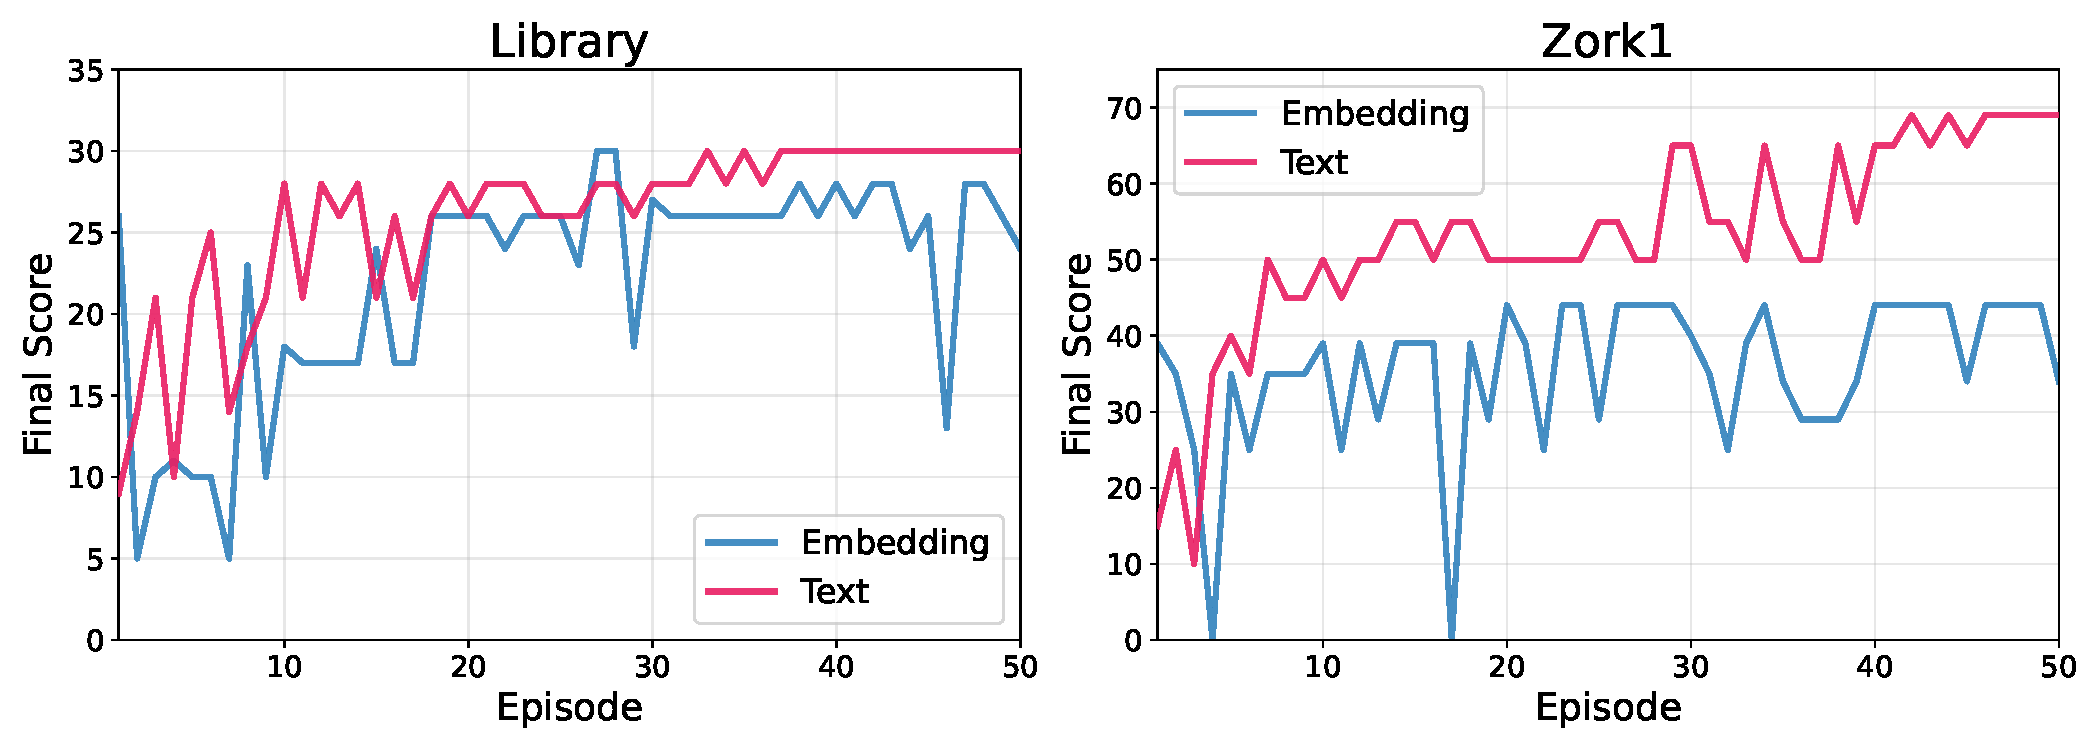
\includegraphics[width=\columnwidth, page=1]{figures/memory_vs_jitrl.pdf}
    \vspace{-3mm}
    \caption{Performance Comparison of Text-based and Embedding-based State Representations.}
    \vspace{-3mm}
    \label{fig:embedding}
\end{figure}
We compare our structured text state summary (\textbf{Text}) against state embedding (\textbf{Embedding}) on Library and Zork1. Figure~\ref {fig:embedding} shows that the Text achieves superior stability and performance, whereas Embedding exhibits significant fluctuation. We attribute this to the low discriminative power of dense embeddings in text games; they often assign high similarity to topologically distinct but descriptively similar states. This ambiguity leads to the retrieval of mismatched memories, introducing noise that degrades policy improvement.

\section{Step Analysis}


\begin{table}[t]
  \caption{Average Steps per Website.}
  \vskip 0.1in
  \label{tab:avg_steps_per_site}
  \begin{center}
    \begin{small}
      \begin{tabular}{lcccccc}
        \toprule
        \textbf{Website} 
        & \textbf{GitLab} 
        & \textbf{Map} 
        & \textbf{Reddit} 
        & \textbf{Shopping} 
        & \textbf{Admin}
        & \textbf{Overall} \\
        \midrule
        \textbf{Avg Steps} 
        & 5.83 
        & 9.39 
        & 4.57 
        & 5.55 
        & 6.20
        & \textbf{6.28} \\
        \bottomrule
      \end{tabular}
    \end{small}
  \end{center}
  \vskip -0.1in
\end{table}


Table~\ref{tab:avg_steps_per_site} presents the average number of steps required by the agent to complete tasks across different website domains. The results reveal notable differences in task complexity among the domains. The Map website poses the greatest challenge, requiring an average of 9.39 steps per task, as map-based navigation typically involves sequential operations such as searching locations, adjusting views, and extracting information. In contrast, Reddit and Admin websites present relatively simpler navigation patterns, averaging only 4.57 and 5.55 steps, respectively, as these platforms often allow more direct access to target content. 


% \section{Ablation on Exploration Rate $\lambda$}
% \label{app:ablation_lambda}

% We ablate the exploration rate $\lambda$ on both Jericho (three games: Library, Zork1, Zork3; averaged over 50 episodes) and WebArena (five website domains; averaged over 5 episodes per task). We vary $\lambda \in \{0, 0.25, 0.50, 0.65, 0.75\}$ for Jericho and $\lambda \in \{0, 0.05, 0.25, 0.50, 0.75\}$ for WebArena, keeping all other hyperparameters fixed. As shown in Tables~\ref{tab:ablation_lambda_jericho} and~\ref{tab:ablation_lambda_webarena}, performance is stable across a reasonable range of both parameters. WebArena favors a smaller $\lambda$ since its structured action space requires less exploration, while Jericho benefits from a larger $\lambda$ due to its combinatorially large action space, where extensive exploration is essential to discover effective action sequences.

% \begin{table}[h]
% \centering
% \caption{Ablation of $\lambda$ on Jericho (Avg score over 50 episodes).}
% \label{tab:ablation_lambda_jericho}
% \vskip 0.1in
% \begin{tabular}{lccc}
% \toprule
% $\lambda$ & \textbf{Library} & \textbf{Zork1} & \textbf{Zork3} \\
% \midrule
% 0    & 20.8 & 42.1 & 2.1 \\
% 0.25 & 24.1 & 48.6 & 2.6 \\
% 0.50 & 24.9 & \textbf{52.7} & \textbf{3.1} \\
% \textbf{0.65} & \textbf{25.9} & 53.0 & \textbf{3.1} \\
% 0.75 & 25.7 & 51.4 & 2.9 \\
% \bottomrule
% \end{tabular}
% \end{table}

% \begin{table}[h]
% \centering
% \caption{Ablation of $\lambda$ on WebArena (Avg success rate \%, full).}
% \label{tab:ablation_lambda_webarena}
% \vskip 0.1in
% \begin{tabular}{lcccccc}
% \toprule
% $\lambda$ & \textbf{Admin} & \textbf{GitLab} & \textbf{Map} & \textbf{Reddit} & \textbf{Shopping} & \textbf{Average} \\
% \midrule
% 0    & 50.77 & 39.51 & 36.41 & 55.81 & 40.42 & 45.38 \\
% \textbf{0.05} & 52.31 & 40.78 & \textbf{37.66} & 57.64 & \textbf{41.67} & \textbf{46.98} \\
% 0.25 & \textbf{52.75} & \textbf{41.18} & 37.19 & \textbf{57.89} & 41.25 & 46.52 \\
% 0.50 & 49.01 & 38.04 & 34.38 & 53.49 & 37.08 & 43.36 \\
% 0.75 & 46.15 & 36.27 & 32.81 & 51.94 & 35.42 & 41.32 \\
% \bottomrule
% \end{tabular}
% \end{table}

% \section{Sensitivity to UCB Bonus $\alpha$}
% \label{app:ablation_alpha}

% We ablate the UCB bonus $\alpha$ on both Jericho (three games: Library, Zork1, Zork3; averaged over 50 episodes) and WebArena (five website domains; averaged over 5 episodes per task), varying $\alpha \in \{3, 5, 7, 10\}$ while keeping all other hyperparameters fixed. As shown in Tables~\ref{tab:ablation_alpha_jericho} and~\ref{tab:ablation_alpha_webarena}, performance is stable across a reasonable range of $\alpha$, with $\alpha = 5$ achieving the best overall balance between exploration incentive and over-optimism.

% \begin{table}[h]
% \centering
% \caption{Sensitivity of $\alpha$ on Jericho (Avg score over 50 episodes).}
% \label{tab:ablation_alpha_jericho}
% \vskip 0.1in
% \begin{tabular}{lccc}
% \toprule
% $\alpha$ & \textbf{Library} & \textbf{Zork1} & \textbf{Zork3} \\
% \midrule
% 3  & 23.8 & 50.5 & 2.7 \\
% \textbf{5}  & \textbf{25.9} & 53.0 & \textbf{3.1} \\
% 7  & 24.6 & \textbf{54.2} & 2.8 \\
% 10 & 23.4 & 49.2 & 2.6 \\
% \bottomrule
% \end{tabular}
% \end{table}

% \begin{table}[h]
% \centering
% \caption{Sensitivity of $\alpha$ on WebArena (Avg success rate \%).}
% \label{tab:ablation_alpha_webarena}
% \vskip 0.1in
% \begin{tabular}{lccccc}
% \toprule
% $\alpha$ & \textbf{Admin} & \textbf{GitLab} & \textbf{Map} & \textbf{Reddit} & \textbf{Shopping} \\
% \midrule
% 3  & \textbf{53.48} & 39.80 & 35.78 & \textbf{58.45} & 40.52 \\
% \textbf{5}  & 52.31 & \textbf{40.78} & \textbf{37.66} & 57.64 & \textbf{41.67} \\
% 7  & 49.02 & 39.22 & 34.50 & 55.04 & 38.54 \\
% 10 & 46.52 & 37.45 & 33.03 & 53.02 & 36.98 \\
% \bottomrule
% \end{tabular}
% \end{table}

\section{Scalability of JitRL}
\label{app:scalability}

We evaluate JitRL's scalability on the Library game from Jericho over 50 episodes, measuring how retrieval latency and average game score evolve as the memory bank grows. We partition the memory into bins of 500 entries and report the average retrieval time (in milliseconds) and average score within each bin. As shown in Table~\ref{tab:scalability}, JitRL's performance continuously improves as memory grows, while retrieval overhead remains negligible compared to LLM inference time.

\begin{table}[h]
\centering
\caption{Inference overhead and performance as memory grows (Library, 50 episodes).}
\label{tab:scalability}
\vskip 0.1in
\begin{tabular}{lcc}
\toprule
\textbf{Memory Size (\# entries)} & \textbf{Retrieval (ms)} & \textbf{Avg Score} \\
\midrule
0--500    & 15--22 & 18.1 \\
500--1000  & 26--27 & 25.1 \\
1000--1500 & 29     & 27.2 \\
1500--2000 & 38     & 29.2 \\
2000--2500 & 47     & 30.0 \\
\bottomrule
\end{tabular}
\end{table}

\section{GRPO Hyperparameter Sweep and Comparison with JitRL}
\label{app:grpo_sweep}

\subsection{Clarification on Rollout Count vs.\ Batch Size}

In GRPO, each problem instance is rolled out $G$ times, and the advantage for each trajectory is computed via group-relative normalization over all trajectories sharing the same instance:
\begin{equation}
    \hat{A}_i = \frac{r_i - \mathrm{mean}(\{r_j\}_{j \in \text{group}})}{\mathrm{std}(\{r_j\}_{j \in \text{group}})}.
\end{equation}
Since all training data in our Jericho setting originates from the same initial game observation (analogous to a single prompt), increasing rollout count $G$ and increasing batch size both raise the total number of trajectories per gradient step, but differ in the scope of group normalization:

\begin{itemize}[leftmargin=*,nosep]
    \item \textbf{Increasing rollout count} (e.g., $G{=}64$, batch size${=}1$): All 64 trajectories share one group ID, so group-relative normalization is performed jointly over all 64 trajectories, yielding a smoother advantage estimate.
    \item \textbf{Increasing batch size} (e.g., $G{=}8$, batch size${=}8$): Each copy of the instance receives an independent group ID, creating 8 independent groups of 8 rollouts. Normalization is performed within each group of 8, making the advantage more sensitive to local variation.
\end{itemize}

\subsection{Experimental Setup}

We conduct experiments on Zork1 using Qwen3-32B (bf16) trained with GRPO for 50 training steps, matching the number of episodes used in JitRL evaluation. After each training step, we evaluate the model with a single rollout and record the score. We sweep four hyperparameters — rollout count $G$, batch size, PPO epochs, and learning rate — varying one axis at a time while fixing the others. All experiments are run on 4$\times$ NVIDIA H200 GPUs with tensor parallelism of 4, a maximum of 80 turns per episode, a maximum response length of 8,192 tokens, and KL coefficient 0.001 (low-variance KL).

\subsection{Results}

Table~\ref{tab:grpo_sweep} summarizes the validation mean, max, and min scores across all swept configurations, along with the total number of training episodes consumed by each setting.

\begin{table}[h]
\centering
\caption{GRPO hyperparameter sweep on Zork1 (Qwen3-32B, 50 training steps).}
\label{tab:grpo_sweep}
\vskip 0.1in
\begin{tabular}{ccccccc}
\toprule
\textbf{Rollout} & \textbf{Batch Size} & \textbf{PPO Epochs} & \textbf{LR} & \textbf{Val Mean} & \textbf{Val Max} & \textbf{Val Min} \\
\midrule
8  & 1 & 1 & 1e-6 & 16.2 & 35 & 0  \\
16 & 1 & 1 & 1e-6 & 13.6 & 40 & 0  \\
32 & 1 & 1 & 1e-6 & 12.0 & 40 & -5 \\
8  & 1 & 2 & 1e-6 & 10.4 & 40 & 0  \\
8  & 1 & 4 & 1e-6 & 17.1 & 40 & 5  \\
8  & 1 & 4 & 1e-5 & 25.5 & 45 & -5 \\
\textbf{8}  & \textbf{8} & \textbf{1} & \textbf{1e-5} & \textbf{40.7} & \textbf{55} & 5  \\
\bottomrule
\end{tabular}
\end{table}

\subsection{Analysis}

As shown in Table~\ref{tab:grpo_sweep}, the best GRPO configuration (rollout${=}8$, batch size${=}8$, PPO epochs${=}1$, lr${=}$1e-5) achieves a mean validation score of 40.7 and a maximum of 55 on Zork1, with a clear upward learning curve that stabilizes near 55 in the final 20 steps. This is competitive with JitRL's mean score of 53.0 using the same Qwen3-32B backbone.

However, this result comes at a substantial sample cost. Over 50 steps, JitRL requires exactly \textbf{50 trajectories} in total. In contrast, GRPO consumes $50 \times G \times \text{batch size}$ trajectories per run. The best GRPO configuration alone requires \textbf{3,200 training episodes} — over \textbf{64$\times$ more} than JitRL. Even the original GRPO setting reported in the main paper (rollout${=}8$, batch size${=}1$) requires 400 episodes, \textbf{8$\times$ more} than JitRL. While GRPO with extensive hyperparameter tuning can approach JitRL's performance, this comes at a substantially higher sample cost, further highlighting JitRL's efficiency advantage.

\section{Cost Analysis.}
\label{app:cost}
%The training of \textbf{WebRL}, based on the \texttt{Llama-3.1-70B-Instruct} backbone, requires approximately 156.5 hours of computation on an 16 $\times$ NVIDIA H200 GPU cluster. This intensive process is divided into several stages: the initial Supervised Fine-Tuning (SFT) phase accounts for 65 hours, followed by the Rollout and Interaction phase for trajectory generation at 52 hours. The final stages, consisting of Reward Labeling and Actor-Critic Optimization, require 1 hour and 38.5 hours, respectively. Based on a standard market rate of \$32 per node-hour, the total estimated expenditure for a single complete training cycle is approximately \$5,008, reflecting the significant capital investment required for high-fidelity web-agent alignment at this scale. 
The training of \textbf{WEBRL}, based on the \texttt{Llama-3.1-70B-Instruct} backbone, requires approximately 154 hours of computation on a 16 $\times$ NVIDIA H200 GPU cluster (distributed across 2 nodes). This intensive online reinforcement learning process is structured into two primary stages: the initial Supervised Fine-Tuning (SFT) phase, which accounts for 10 hours to establish foundational web-navigation capabilities, followed by an iterative 8-phase Reinforcement Learning cycle. Within each RL phase, the Self-Evolving Task Generation and Filtering requires 8 hours (1 hour per phase), while the Online Rollout and Interaction phase for generating trajectories takes approximately 48 hours (6 hours per phase). The Reward Labeling (utilizing an 8B ORM) and the heavy Actor-Critic Optimization (managing 70B parameters with a 16,384 cutoff length) require 2 hours (15 mins per phase) and 86 hours (10.75 hours per phase), respectively. Based on a standard market rate of \$64 per hour for 2 nodes, the total estimated expenditure for a single complete 70B training cycle is approximately \$9,856.
The operational costs for JitRL and other training-free baselines are calculated based on token consumption through the OpenRouter API, which serves as the uniform billing standard for these inference-based methods.